%%%%%%%%%%%%%%%%%%%%%%%%%%%%%%%%%%%%%%%%%%%%%%%%%%%%%%
% A Beamer template for University of Wollongong     %
% Based on THU beamer theme                          %
% Author: Qiuyu Lu                                   %
% Date: July 2024                                    %
% LPPL Licensed.                                     %
%%%%%%%%%%%%%%%%%%%%%%%%%%%%%%%%%%%%%%%%%%%%%%%%%%%%%%
% Customized for Sharif University of Technology     %
%%%%%%%%%%%%%%%%%%%%%%%%%%%%%%%%%%%%%%%%%%%%%%%%%%%%%%


\documentclass[serif, aspectratio=169]{beamer}
%\documentclass[serif]{beamer}  % for 4:3 ratio
\usepackage[T1]{fontenc} 
\usepackage{fourier} % see "http://faq.ktug.org/wiki/uploads/MathFonts.pdf" for other options
\usepackage{hyperref}
\usepackage{latexsym,amsmath,xcolor,multicol,booktabs,calligra}
\usepackage{graphicx,pstricks,listings,stackengine}
\usepackage{lipsum}
\usepackage{tikz}
\usetikzlibrary{shapes.geometric} % Add this to include ellipse shapes
\usepackage{amsmath}
\usepackage{pgfplots}  % For plots
\usepackage{amsmath}   % For equations
\usepackage{array}     % For tables
\pgfplotsset{compat=1.16}

% \usetikzlibrary{positioning}


\author{Ali Sharifi-Zarchi}
\title{Machine Learning (CE 40717)}
\subtitle{Fall 2024}
\institute{
    CE Department \\
    Sharif University of Technology
}
%\date{\small \today}
% \usepackage{UoWstyle}
\usepackage{SUTstyle}

% defs
\def\cmd#1{\texttt{\color{red}\footnotesize $\backslash$#1}}
\def\env#1{\texttt{\color{blue}\footnotesize #1}}
\definecolor{deepblue}{rgb}{0,0,0.5}
\definecolor{deepred}{RGB}{153,0,0}
\definecolor{deepgreen}{rgb}{0,0.5,0}
\definecolor{halfgray}{gray}{0.55}

\lstset{
    basicstyle=\ttfamily\small,
    keywordstyle=\bfseries\color{deepblue},
    emphstyle=\ttfamily\color{deepred},    % Custom highlighting style
    stringstyle=\color{deepgreen},
    numbers=left,
    numberstyle=\small\color{halfgray},
    rulesepcolor=\color{red!20!green!20!blue!20},
    frame=shadowbox,
}

\begin{document}

\begin{frame}
    \titlepage
    \vspace*{-0.6cm}
    \begin{figure}[htpb]
        \begin{center}
            
\includegraphics[keepaspectratio, scale=0.25]{pic/sharif-main-logo.png}
        \end{center}
    \end{figure}
\end{frame}

\begin{frame}    
\tableofcontents[sectionstyle=show,
subsectionstyle=show/shaded/hide,
subsubsectionstyle=show/shaded/hide]
\end{frame}

% ============================ Introduction ============================ 
\section{Introduction}

\begin{frame}{Perceptron Reminder}
    \begin{picture}(0,0)
            \put(200,-150){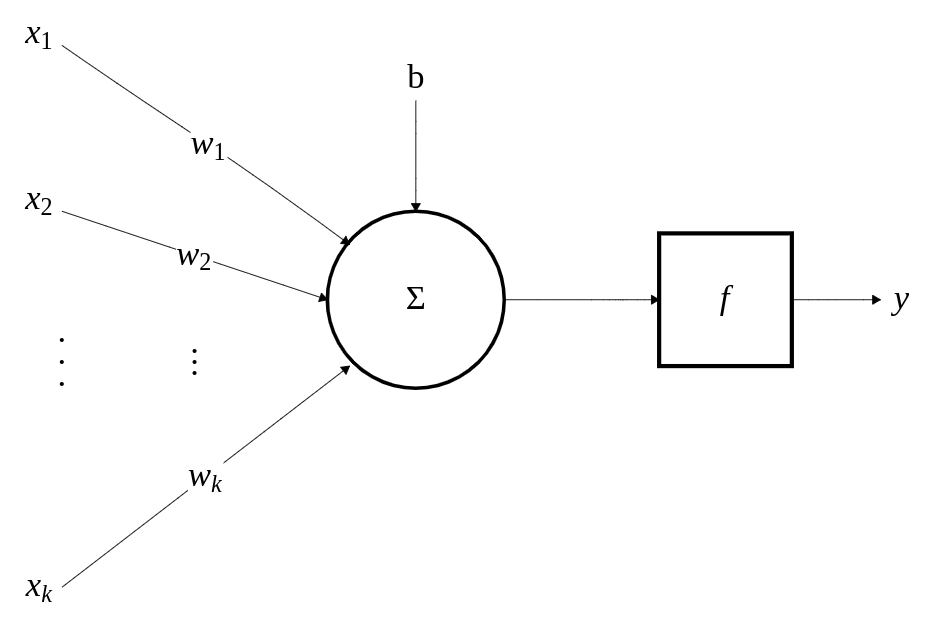
\includegraphics[width=7cm]{pic/1/neuron.png}} % Adjust path and size
    \end{picture}
    The building block of each neural network is Perceptron:
    \begin{itemize}
        \item $\{x_1, x_2, \dots, x_k\}$ : input features
        \item $\{w_1, w_2, \dots, w_k\}$ : feature weights
        \item $b$ : bias term
        \item $f(\cdot)$ : activation function
        \item $y$ : output of the neuron
    \end{itemize}
\end{frame}


\begin{frame}[t]{Perceptron Capacity}
\begin{figure}[h]
        \centering
        \begin{minipage}{0.45\textwidth}
            \begin{itemize}
                \item A perceptron solves linearly separable problems
                \item The XOR gate is not linearly separable
                \item We need a multi-layer perceptron for such problems
            \end{itemize}
        \end{minipage}
        \hfill
        \begin{minipage}{0.45\textwidth}
            \centering
            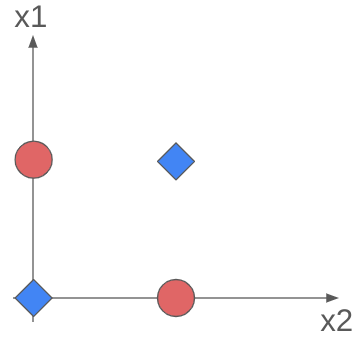
\includegraphics[width=\textwidth]{pic/1/xor.png}
            {\scriptsize XOR gate}
        \end{minipage}
    \end{figure}
\end{frame}


\begin{frame}{Why Neural Networks?}
    \begin{itemize}
        \item We can find explicit formulas for some problems (no machine learning)
        \begin{itemize}
            \item $\Delta x = \dfrac{1}{2}a\cdot t^2 + v_0 \cdot t$
        \end{itemize}
        \item We can model some problems assuming simple relationships (classical machine learning)
        \begin{itemize}
            \item House price as a linear function of its features
            \item $y = a_1 \cdot x_1 + a_2 \cdot x_2 + \ldots + a_p \cdot x_p$
        \end{itemize}
        \item How about classifying these images?
        \begin{center}
            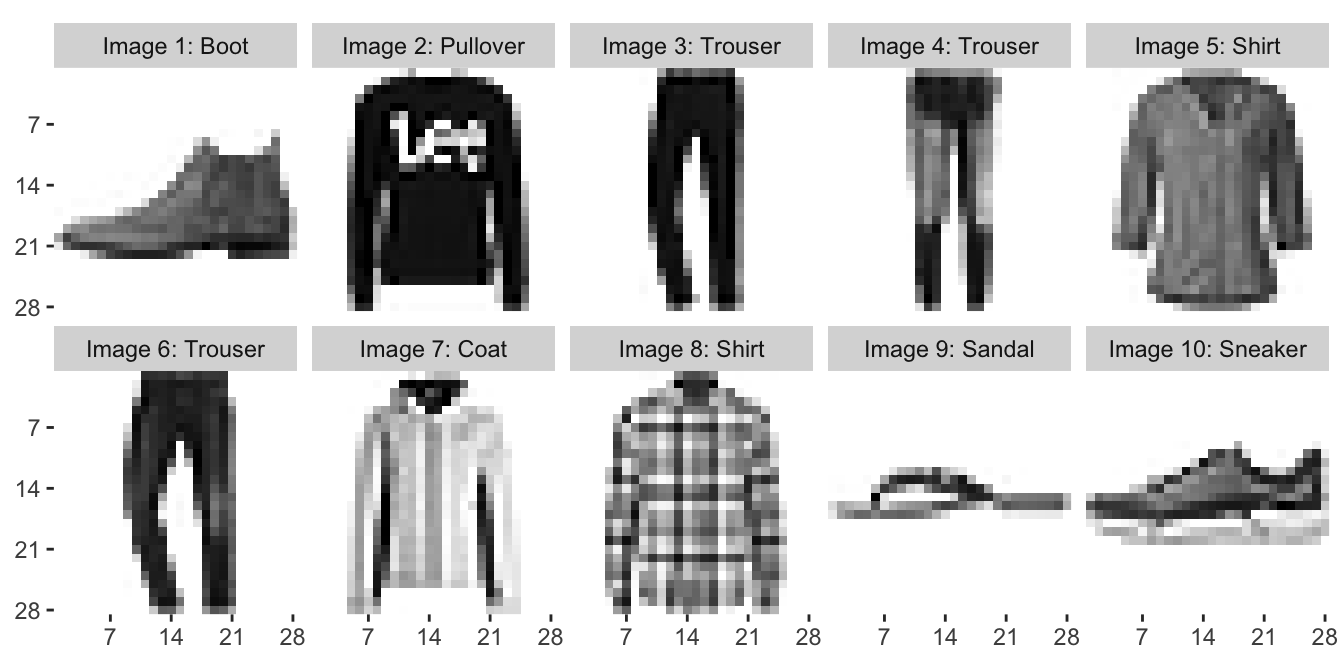
\includegraphics[keepaspectratio, scale=0.1]{pic/1/fashion-mnist.png}
        \end{center}
    \end{itemize}
\end{frame}


\begin{frame}[t]{Why Neural Networks? Cont.}
    \begin{picture}(0,0)
            \put(200, -150){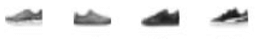
\includegraphics[width=7cm]{pic/1/sneakers.png}}
    \end{picture}
    
    \begin{itemize}
        \item No explicit formula exists to recognize a sneaker
        \item We recognize any sneaker intuitively
        \item Our brains use a complex function for this recognition
        \item \textbf{Deep neural networks} can learn this complex function
    \end{itemize}
\end{frame}

%
\section{Multi-Layer Perceptron (MLP)}

\begin{frame}{Example: MLP for Complex Patterns}
    \begin{itemize}
        \item What network to learn this area?
        \item Example is adapted from [1].
        \begin{figure}[htpb]
        \begin{center}
            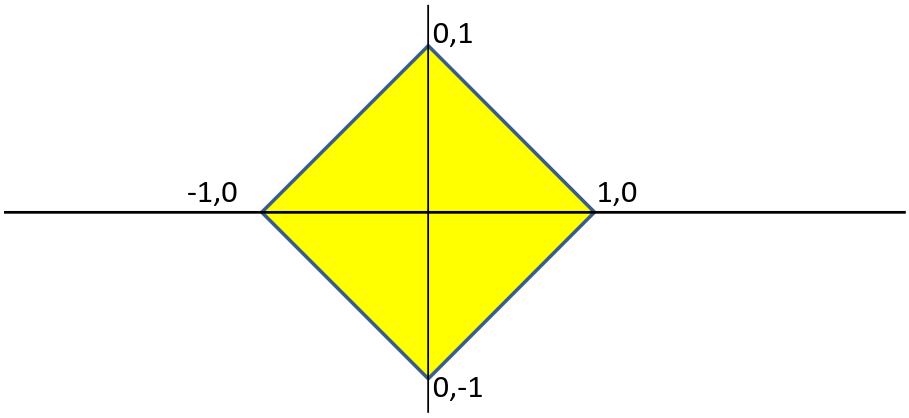
\includegraphics[keepaspectratio, scale=0.25]{pic/2/ex1.png}
        \end{center}
    \end{figure}
    \end{itemize}
\end{frame}


\begin{frame}{Example: MLP for Complex Patterns Cont.}
        \begin{figure}[htpb]
        \begin{center}
            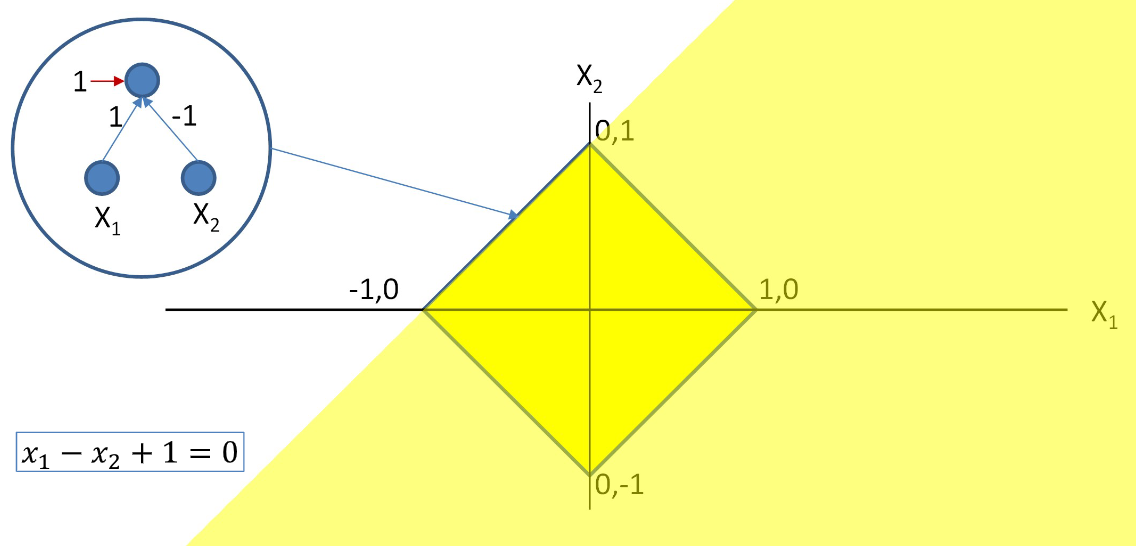
\includegraphics[keepaspectratio, scale=0.25]{pic/2/ex2.png}
        \end{center}
    \end{figure}
\end{frame}


\begin{frame}{Example: MLP for Complex Patterns Cont.}
        \begin{figure}[htpb]
        \begin{center}
            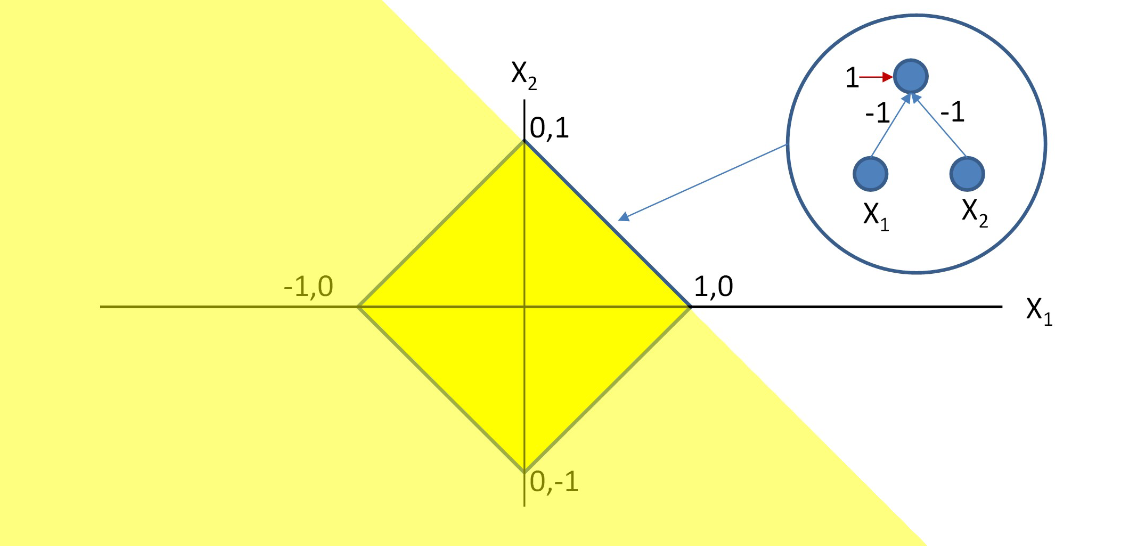
\includegraphics[keepaspectratio, scale=0.25]{pic/2/ex3.png}
        \end{center}
    \end{figure}
\end{frame}


\begin{frame}{Example: MLP for Complex Patterns Cont.}
        \begin{figure}[htpb]
        \begin{center}
            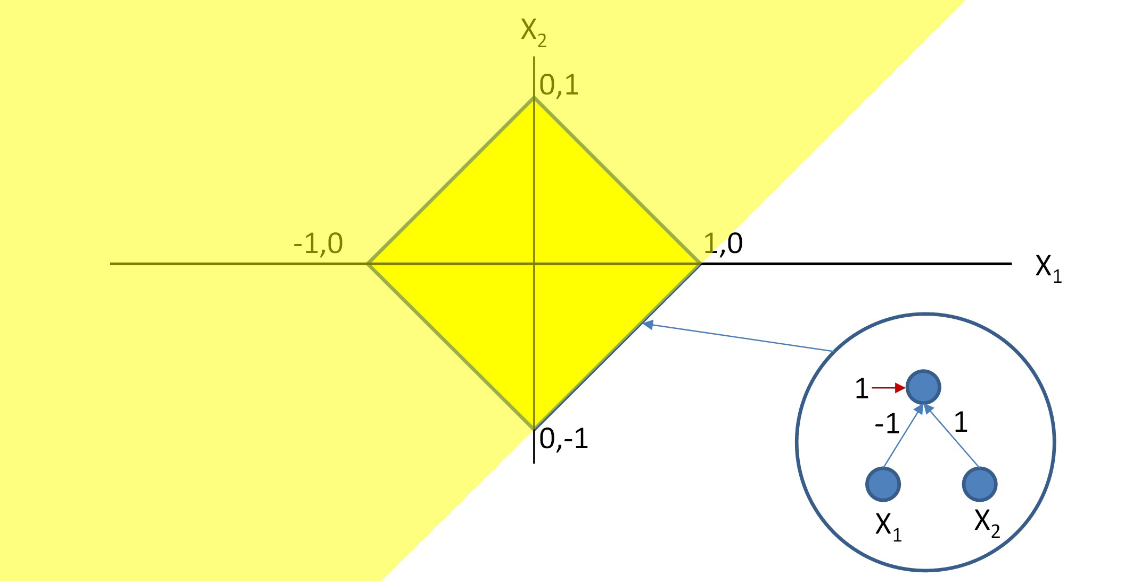
\includegraphics[keepaspectratio, scale=0.25]{pic/2/ex4.png}
        \end{center}
    \end{figure}
\end{frame}


\begin{frame}{Example: MLP for Complex Patterns Cont.}
        \begin{figure}[htpb]
        \begin{center}
            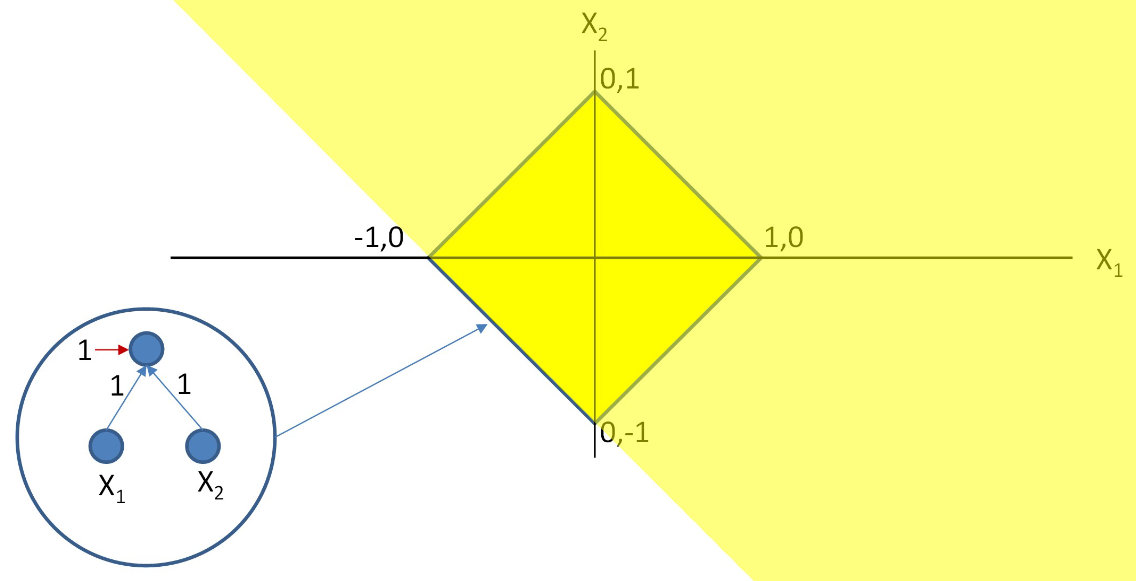
\includegraphics[keepaspectratio, scale=0.25]{pic/2/ex5.png}
        \end{center}
    \end{figure}
\end{frame}


\begin{frame}{Example: MLP for Complex Patterns Cont.}
        \begin{figure}[htpb]
        \begin{center}
            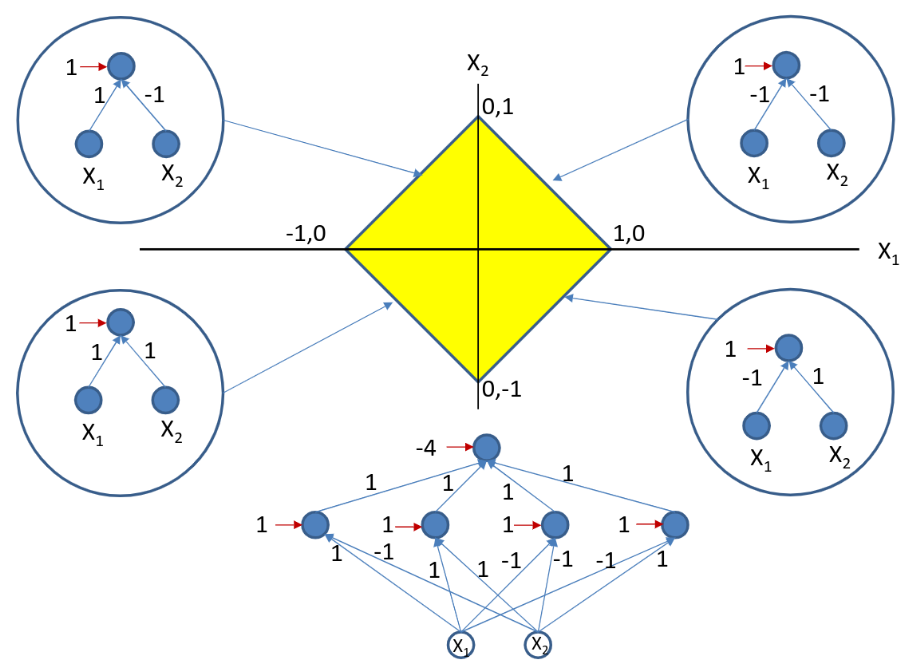
\includegraphics[keepaspectratio, scale=0.25]{pic/2/ex6.png}
        \end{center}
    \end{figure}
\end{frame}

\begin{frame}{MLP Capacity}
    \begin{columns}
        \begin{column}{0.6\textwidth}
            \begin{itemize}
                \item Increasing width and depth allows us to approximate complex decision boundaries
                \item An activation function makes a neuron’s output non-linear, allowing the network to learn complex data
                \item Not limited to Boolean or step functions
                \item With appropriate activation functions, neural networks can approximate any real-valued function (More details later)
            \end{itemize}
        \end{column}
        \begin{column}{0.4\textwidth}
            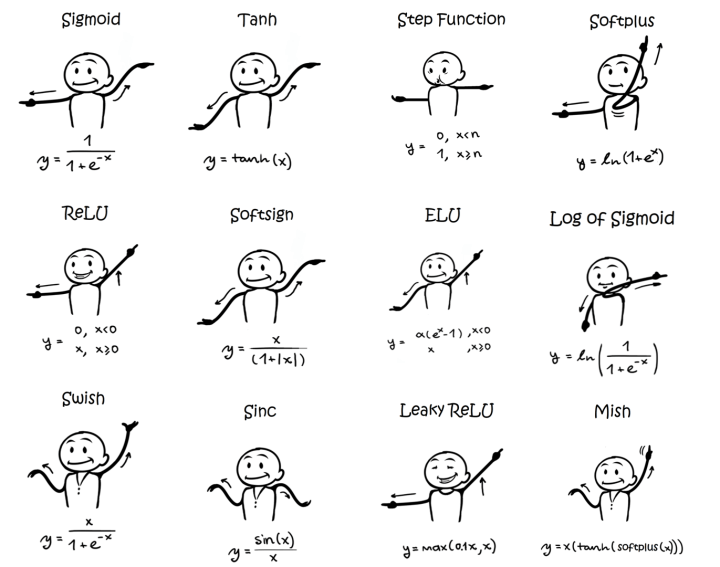
\includegraphics[width=\textwidth]{pic/2/activations.png} \\
            \begin{center}
            {\scriptsize Adapted from \href{https://sefiks.com/2020/02/02/dance-moves-of-deep-learning-activation-functions/}{Sefiks}}
            \end{center}
        \end{column}
    \end{columns}
\end{frame}


\section{Neural Networks}
\begin{frame}{Single Hidden Layer Neural Network}
    \minipage{.5\textwidth}
    \begin{itemize}
        \item Hidden layer pre-activation:
        $$a(x)_i = b^{(1)}_i + \sum_j W^{(1)}_{ij} \cdot x_j$$
        \item Activated hidden layer:
        $$h(x) = f(a(x))$$
        \item Output layer:
        $$ o(x) = o\left(b^{(2)} + W^{(2)}h^{(1)}x \right) $$
    \end{itemize}
    \endminipage
    \hfill
    \minipage{.48\textwidth}
        \begin{figure}[bh]
            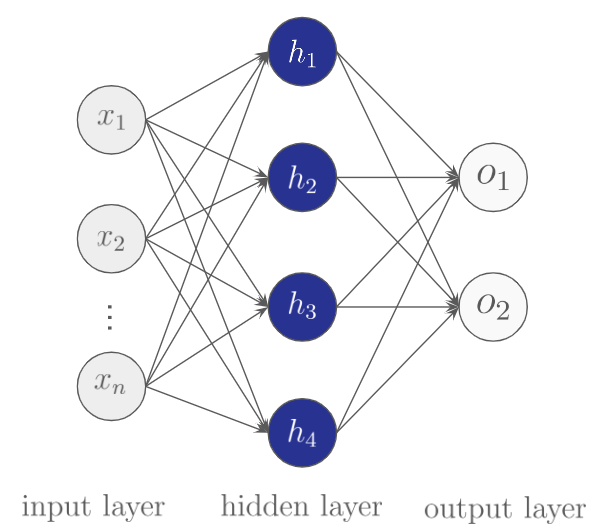
\includegraphics[width=\linewidth]{pic/2/single-hidden_nn.png}
        \end{figure}
    \endminipage
\end{frame}


\begin{frame}{Multi-Hidden Layer Neural Network}
    \minipage{.4\textwidth}
    \begin{itemize}
        \item Let $h^0_i = x_i$ for $i \in \{1, 2, \ldots, n  \}$
        \item For $\ell \in \{0, 1, \ldots, L \}$:
        $$a^{(\ell+1)}_j = b^{(\ell)}_j + \sum_i W^{(\ell)}_{ij}\cdot h^{(\ell)}_i$$
        $$h^{(\ell+1)}_j = f(a^{(\ell+1)}_j)$$

        \item Learnable parameters:
        $$b^{(\ell)}_j, W^{(\ell)}_{ij}$$

        \item Number of learnable parameters:
        $$(n+1)m_1 + (m_1 + 1)m_2 + ... + (m_L + 1)k$$
    \end{itemize}
    \endminipage
    \hfill
    \minipage{.6\textwidth}
        \begin{figure}[bh]
            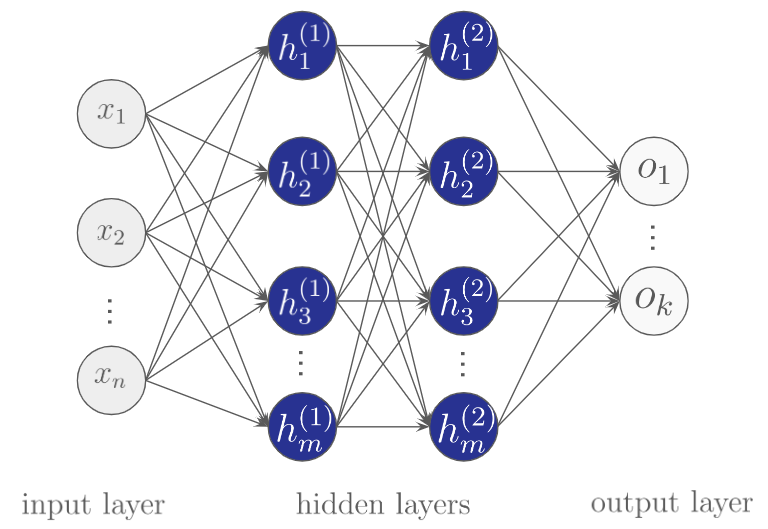
\includegraphics[width=\linewidth]{pic/2/multi-hidden-nn.png}
        \end{figure}
    \endminipage
\end{frame}

\begin{frame}[t]{Deep Neural Network Architecture}
\begin{itemize}
    \item More than a few hidden layers: Deep Neural Network (DNN)
    \item Designing a neural network architecture is more of an art than a science.
        \begin{figure}[bh]
            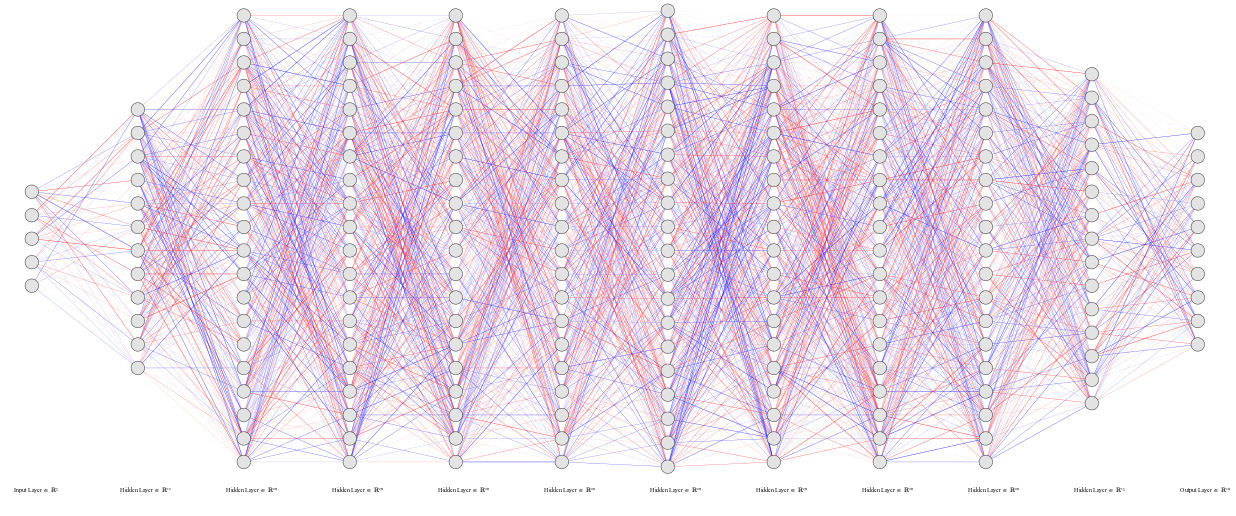
\includegraphics[keepaspectratio, scale=0.3]{pic/3/huge-nn.png}
        \end{figure}
\end{itemize}
\end{frame}

\begin{frame}[t]{Network Width and Depth}
    \begin{columns}
        \begin{column}{0.6\textwidth}
            \begin{itemize}
                \item \textbf{Width:} More neurons, more complexity
                \item \textbf{Depth:} More layers, more abstraction
                \item \textbf{Balance:} 
                \begin{itemize}
                    \item Too narrow/shallow: risk of underfitting
                    \item Too wide/deep: risk of overfitting
                \end{itemize}
            \end{itemize}
        \end{column}
        \begin{column}{0.5\textwidth}
            \begin{center}
                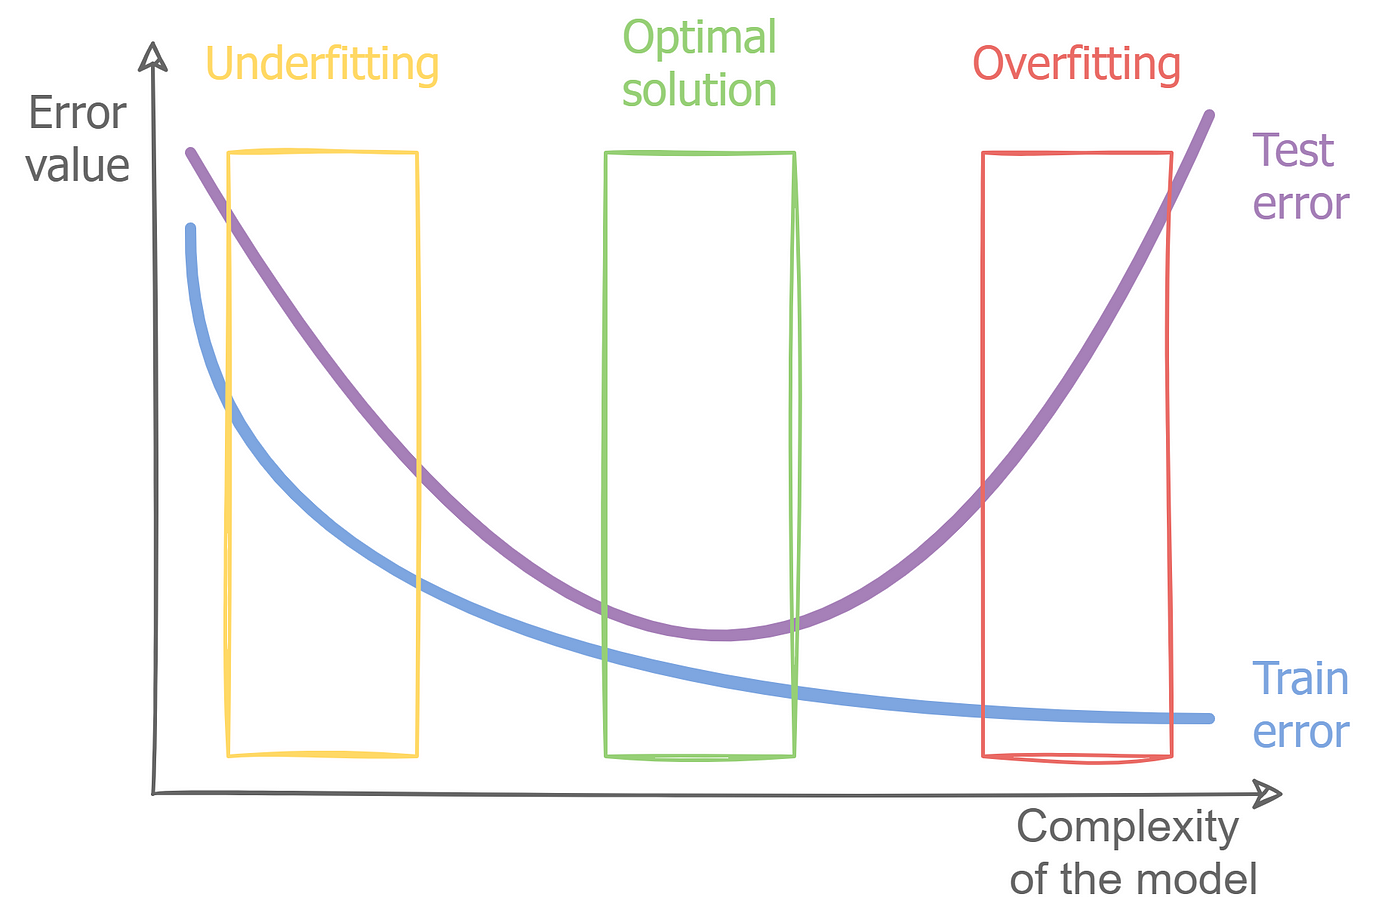
\includegraphics[keepaspectratio, width=\textwidth]{pic/3/complexity.png} \\
                {\scriptsize Adapted from \href{https://towardsdatascience.com/overfitting-and-underfitting-principles-ea8964d9c45c}{Towards Data Science}}
            \end{center}
        \end{column}
    \end{columns}
\end{frame}

\section{Training Neural Networks}
\begin{frame}{Training Phases}
    \begin{itemize}
        \item \textbf{Initialize weights and biases}: These values control how the network initially processes information (More details later)
        \item \textbf{Forward pass}: Pass the input through the network to get an output
        \item \textbf{Calculate the error}: Compare the network's output to the correct answer to measure the difference (called the 'loss' - More details later) 
        \item \textbf{Backpropagation}: Use the loss value to adjust the weights and biases to improve the network's accuracy
    \end{itemize}
    \begin{figure}[bh]
            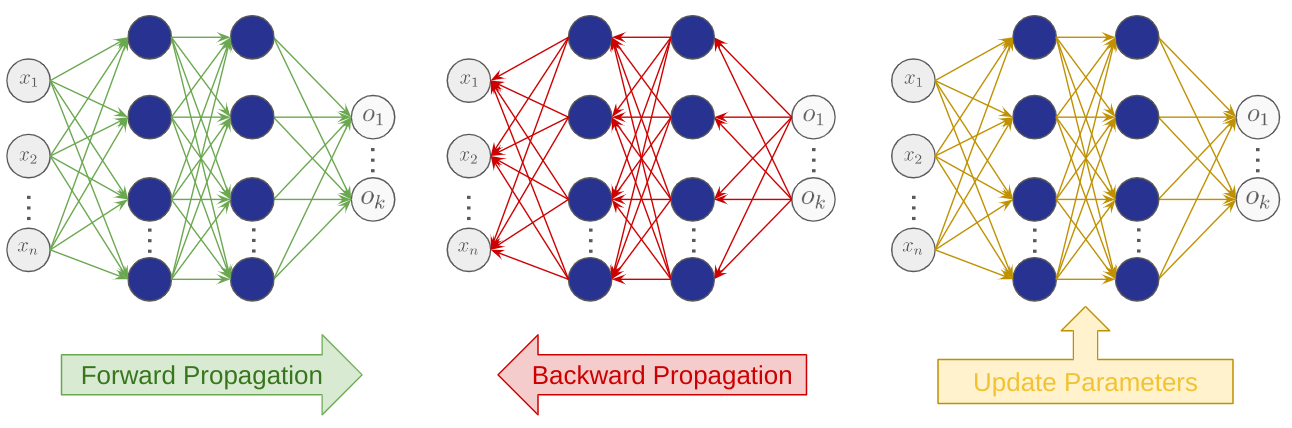
\includegraphics[keepaspectratio, scale=0.2]{pic/4/training-phases.png}
    \end{figure}
\end{frame}

\begin{frame}[t]{Forward Propagation}
    \begin{itemize}
        \item This is the pass where we send input data through the network to make a prediction (likely inaccurate at first).
        \item The prediction is made by calculating weighted sums and applying an activation function at each layer
        $$ o = a^{(L)} = f^{(L)}\left( b^{(L)} + W^{(L)} \cdot f^{(L-1)}\left( \ldots f^{(1)}(b^{(1)} + W^{(1)x})  \ldots \right) \right) $$
    \end{itemize}
\end{frame}

\begin{frame}{Forward Propagation Cont.}
    \minipage{.45\textwidth}
        \begin{figure}[bh]
            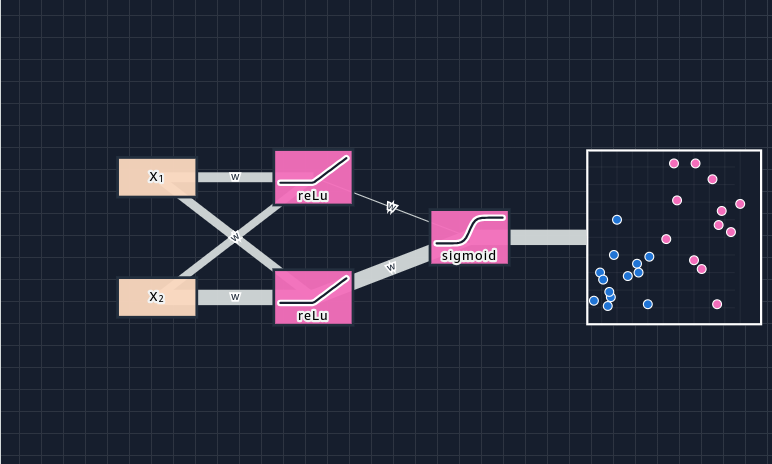
\includegraphics[width=\linewidth]{pic/4/before-forward.png}
            {\scriptsize Before producing predictions. Adapted from \href{https://mlu-explain.github.io/neural-networks/}{mlu-explain}.}
        \end{figure}
    \endminipage
    \hfill
    \minipage{.45\textwidth}
        \begin{figure}[bh]
            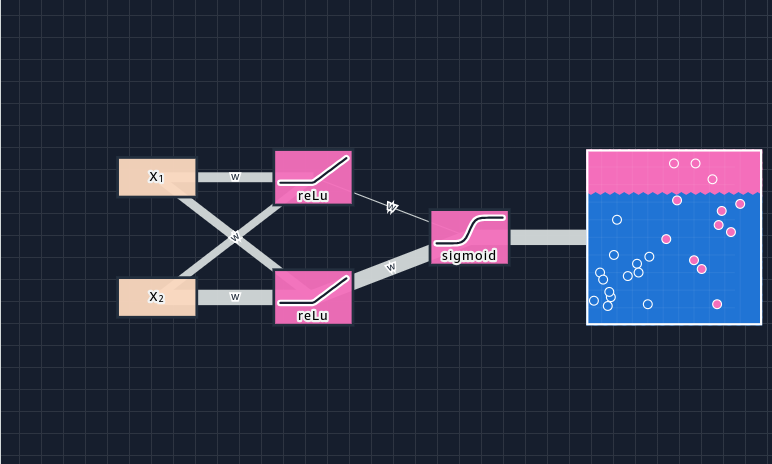
\includegraphics[width=\linewidth]{pic/4/after-forward.png}
            {\scriptsize After producing predictions. Adapted from \href{https://mlu-explain.github.io/neural-networks/}{mlu-explain}.}
        \end{figure}
    \endminipage
\end{frame}


\begin{frame}[t]{Forward Propagation Cont.}
    \begin{itemize}
        \item The goal is to adjust the network’s parameters to improve the predictions
        \item The loss is calculated after the forward pass, telling us how far off our predictions are from the true values
        \begin{figure}[bh]
            \centering
            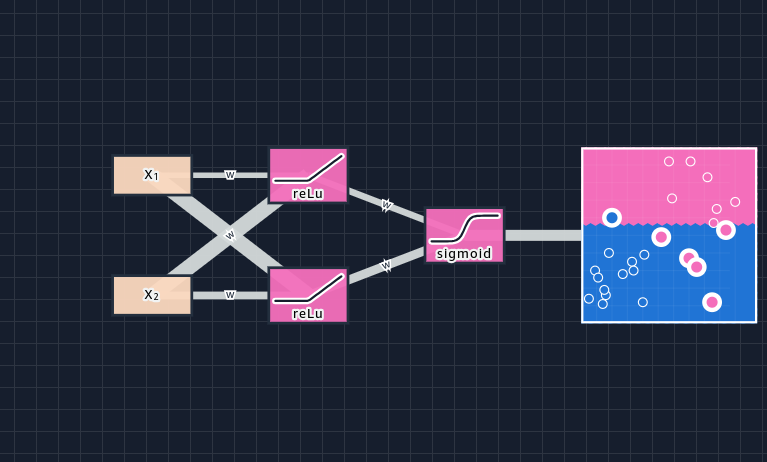
\includegraphics[keepaspectratio, scale=0.25]{pic/4/loss-values.png} \\
            {\scriptsize Loss values for predictions. Adapted from \href{https://mlu-explain.github.io/neural-networks/}{mlu-explain}.}
        \end{figure}
    \end{itemize}
\end{frame}

\begin{frame}[t]{BackPropagation and Parameter Update}
    \begin{itemize}
        \item The network uses the \textbf{loss} to adjust its \textbf{weights and biases} through a process called \textbf{backpropagation}
        \item Backpropagation calculates how much weights should change to reduce the error
        \item This will be explained in more detail in the next lecture
        \begin{figure}[bh]
            \centering
            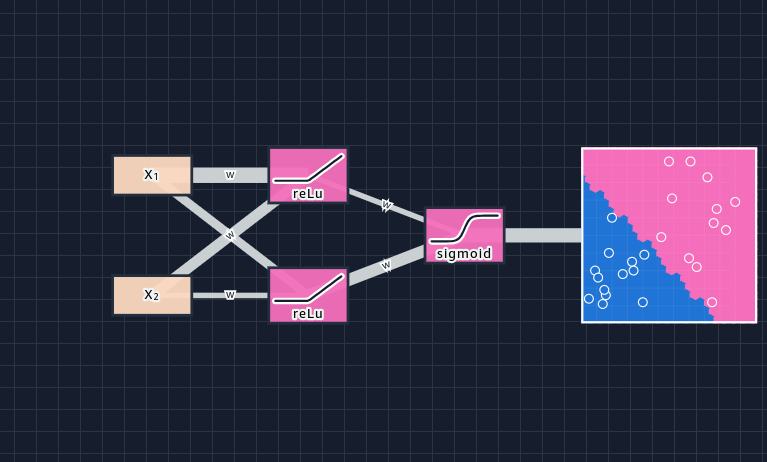
\includegraphics[keepaspectratio, scale=0.25]{pic/4/after-backprop.png} \\
            {\scriptsize Predictions get better as the weights get updated. Adapted from \href{https://mlu-explain.github.io/neural-networks/}{mlu-explain}.}
        \end{figure}
    \end{itemize}
\end{frame}


\section{References}

% \begin{frame}[allowframebreaks]
% \bibliography{ref}
%    \bibliographystyle{ieeetr}
%     \nocite{*} % used here because no citation happens in slides
%    % if there are too many try use:
%     % \tiny\bibliographystyle{alpha}
%  \end{frame}

\end{document}